% Draft for IEEE CASE (conference format, 6 pages + references).
% Every number in this file is copied from the plan/validation records named in
% the "% src:" comments; arithmetic derived from them is marked "% derived".
% Build: see README.md.
\documentclass[conference]{IEEEtran}
\IEEEoverridecommandlockouts
\usepackage{cite}
\usepackage{amsmath,amssymb}
\usepackage{graphicx}
\usepackage{booktabs}
\usepackage{multirow}
\usepackage{algorithm}
\usepackage[noend]{algpseudocode}
\usepackage{xcolor}
\usepackage{tikz}
\usetikzlibrary{arrows.meta,positioning,calc,decorations.pathreplacing,patterns}

\newcommand{\todo}[1]{\textcolor{red}{[TODO: #1]}}
\newcommand{\Qone}{Q1}
\newcommand{\Qtwo}{Q2}
\newcommand{\Qthree}{Q3}
\newcommand{\Qthreep}{Q3p}

\begin{document}

\title{Crossing Queues with Global Re-Ordering for\\
Multi-Forklift Traffic on Free-Form Routes}

\author{\IEEEauthorblockN{\todo{Author names}}
\IEEEauthorblockA{\todo{Affiliation}\\
\todo{e-mail}}}

\maketitle

% src: docs/plans/2026-10-16-fleet-crossing-queues.md (eval700, 117 cells),
%      docs/plans/2026-10-17-fleet-literature-baselines.md (L2-L4, 117 cells),
%      docs/plans/2026-10-17-fleet-large-random-chained.md (r2 + r2x, 36 cells)
\begin{abstract}
Autonomous forklifts on warehouse floors without a fixed roadmap follow
free-form, curvature-constrained routes that touch each other at places nobody
chose in advance. A traffic layer must decide, at every such place, which truck
goes first, without collisions or circular waits, while pedestrians, vehicle
faults, spilled loads, message loss and localization error keep invalidating
the timing it planned with. We present \emph{crossing queues}: every pair of
touching route intervals is a crossing, every truck's interval in it a queue
member with its own ticket, time window and token, and a member that misses
its window rejoins the line at its new free-flow arrival time wherever this
keeps the precedence graph free of cycles. On top of the queues, a
mixed-integer linear program re-orders all still-open crossings every 5\,s to
minimize age-weighted delay, and a speed cap lets a truck arrive as the place
clears. In 117 simulated cells on procedurally generated rack, process and
multi-hall floors with 5--20 trucks and six disturbance conditions, the full
method matched the throughput of a time-window baseline (+0.2\,\%) while
reducing waits longer than 60\,s from 343 to 51 and the longest wait from
540\,s to 124\,s, with no truck--truck overlap and no deadlock. On
1.5$\times$-scaled floors with 20 trucks and chained random jobs it completed
8.3\,\% [1.9, 15.7] more jobs than the baseline and was statistically
indistinguishable from an adapted critical-section coordinator, but its MILP
did not keep up with real time on the larger layouts and two cells collapsed
after the crossing orders locked.
\end{abstract}

\begin{IEEEkeywords}
Multi-robot coordination, AGV traffic management, deadlock avoidance,
mixed-integer programming, warehouse logistics.
\end{IEEEkeywords}

%=============================================================================
\section{Introduction}
%=============================================================================

Fleets of autonomous forklifts are moving into warehouses and plants whose
layouts change and that have no guide paths. When each truck plans its own
curvature-constrained route, e.g., with Hybrid A*~\cite{dolgov2010}, the routes
touch at places that are not known in advance: junctions three routes meet at,
long shared lanes, dead-end aisles a truck enters and leaves again, and reverse
segments. A traffic layer then has to decide, at every such place, which truck
goes first. The decision must keep trucks apart, must never create a circular
wait, and should keep trucks moving, while pedestrians, vehicle faults,
spilled loads, message loss and localization error keep invalidating any
timing it planned with.

Existing approaches differ in what they reserve and how they order.
Zone- and tile-reservation schemes grant space step by step and avoid deadlock
with look-ahead checks~\cite{fransen2022,pratissoli2024,verma2024}.
Critical-section coordinators compute where spatial envelopes overlap and
assign precedence with a heuristic revised every control
period~\cite{pecora2018,mannucci2019,mannucci2021}. Plan-execution graphs keep
the passing order a multi-agent plan implies and are robust to
delay~\cite{honig2016,honig2019,cap2016}; switchable action dependency graphs
re-order such a plan with a MILP on a roadmap~\cite{berndt2024}. Lifelong
multi-agent path finding (MAPF) replans space--time reservations in a rolling
window~\cite{li2021rhcr,varambally2022,bonetti2024}.

Our routes are given and continuous, so we keep them and decide only the
\emph{order in time} at the places where they touch. This paper asks how much
that order is worth and what it costs. Its contributions are:
\begin{enumerate}
\item \emph{Crossing queues} over free-form routes: crossings derived from
  touching route samples, one queue member per truck and crossing with a
  ticket, a time window and a token, and re-queuing of a late member at its
  new free-flow time subject to a lock check (Sec.~\ref{sec:queues}).
\item A \emph{global re-ordering} MILP over all open crossings with an
  age-weighted delay objective, accepted only when the new orders are
  lock-free and lower the planned delay, together with release-time pacing and
  an optional load-dependent physical time model (Sec.~\ref{sec:milp}).
\item An evaluation whose parameters were fixed on development seeds before
  the evaluation seeds were run once: 117 cells on generated floors under six
  disturbance conditions against six other policies, three of them literature
  methods adapted to the same safety layer, and a 36-cell large-scale study
  with paired bootstrap intervals that also reports where the method fails
  (Secs.~\ref{sec:setup}--\ref{sec:results}).
\end{enumerate}

%=============================================================================
\section{Related Work}
%=============================================================================

\emph{Resource reservation.} Fransen et al.~\cite{fransen2022} tessellate the
floor into tiles of any shape and grant a tile reservation only if the
resulting state admits a deadlock-free order of single steps within a
look-ahead; the paper gives worked examples but no tile size or throughput
study. Hierarchical and improved dynamic reservation schemes extend the idea
to industrial layouts~\cite{pratissoli2024,verma2024,digani2015}. Reveliotis
studied MPC traffic scheduling and liveness for zone-controlled guidepath
systems~\cite{reveliotis2018,reveliotis2019}.

\emph{Critical sections and precedence.} The loosely-coupled coordinator of
Pecora et al.~\cite{pecora2018} computes critical sections where two
envelopes overlap, sends each robot a critical point it must not pass, and
orders robots heuristically (e.g., by distance to the section); later work
proves safety under unreliable communication~\cite{mannucci2019} and liveness
with online goals and global re-ordering~\cite{mannucci2021}. Our setting
shares the critical-point idea: a truck receives only the end of its grant.

\emph{Execution graphs.} Temporal plan graphs~\cite{honig2016} and action
dependency graphs (ADG)~\cite{honig2019} execute a MAPF plan by keeping its
passing order, which tolerates arbitrary delays but never re-orders;
RMTRACK~\cite{cap2016} does the same on continuous trajectories. Berndt et
al.~\cite{berndt2024} make the dependencies switchable and re-order them by a
MILP in a receding horizon; every feasible solution is acyclic. Our global
ordering follows the same idea on route-derived crossings, with tokens and
expiry, and without a roadmap. Ordering by alternative graphs in train
rescheduling~\cite{mascis2002,dariano2007} is a further ancestor.

\emph{Lifelong MAPF.} RHCR~\cite{li2021rhcr} resolves collisions only within a
window and replans periodically; RHCRE executes it with an
ADG~\cite{varambally2022}. Prioritized planning with safe
intervals~\cite{phillips2011,cap2015} and fixed-path velocity
tuning~\cite{peng2005} are related. Recent CASE papers apply lifelong MAPF in
plants~\cite{bonetti2024,maoudj2024}, schedule fleets online around executing
robots~\cite{popolizio2024}, and combine reciprocal avoidance with local
MAPF~\cite{dergachev2021}. These assume a grid or roadmap; we compare against
adaptations of three of these families on our fixed routes.

%=============================================================================
\section{System and Problem}
\label{sec:problem}
%=============================================================================

\subsection{Fleet, jobs and routes}
% src: sim/models/dls08_measured/README.md; docs/plans/2026-10-09-fleet-random-worlds.md;
%      docs/plans/2026-10-11-fleet-time-windows.md (stage speeds)
A fleet of $N$ car-like forklifts ($1.46\times0.63$\,m, 24\,kg, measured
small-scale chassis) serves
continuous pallet jobs: from a holding slot, approach and insert into a pallet,
lift, extract, carry it to a drop slot, lower, back out and return to a free
holding slot. Each stage has a cruise speed (approach 0.60, carry 0.30,
extract 0.18, back-out 0.12, insert 0.055\,m/s); lifting and lowering take
4.5\,s each. Routes are planned per truck in space only, with Hybrid
A*~\cite{dolgov2010}, and sampled every 0.1\,m including reverse segments;
all pallet and holding slots other than the truck's own are inflated
planning obstacles, so that a parked truck or a pallet placed later never lies
on an earlier route.

\subsection{Safety layer (common to all policies)}
% src: docs/plans/2026-10-17-fleet-literature-baselines.md (common frame)
A central traffic manager grants each truck $n$ a stretch of its route ahead
of its progress $p_n$, up to a look-ahead of $L=3$\,m. The \emph{claim} of $n$
is the body swept over that stretch, inflated by a margin of 0.3\,m; a grant
is not extended into another truck's body or claim, and the truck brakes to
stop at its grant end. This layer alone keeps trucks apart if they stay within
their grants; the margin covers tracking and localization error. Two recovery
actions run on top of every policy: a detour around a standing truck (TA,
after 20\,s blocked) and a back-off or detour that treats the other truck's
route as a wall (RA, on a wait cycle or after 60\,s blocked)~\todo{cite or
describe internal TA/RA design}.

\subsection{Crossings and the order condition}
% src: docs/plans/2026-10-11-fleet-time-windows.md (sections 1-2)
What the policies decide is who goes first where routes touch. For each pair of
trucks $(a,b)$, the remaining routes are sampled every 0.2\,m with the body
inflated by the margin; touching sample pairs are grouped into maximal
neighbouring clusters, and each cluster is a \emph{crossing} $c$ with an
interval $I_c^a$ on $a$'s route and $I_c^b$ on $b$'s. The same physical place
passed twice (into and out of a dead-end aisle) gives two crossings. An order
$f\prec_c s$ is enforced per sample: $s$ may be granted its sample $k\in
I_c^s$ only after $f$ has passed $\nu_c^s(k)$, the last sample of $I_c^f$
that touches $k$. Crossing and head-on traffic therefore pass one at a time,
while following traffic on the same lane follows at a gap.

\emph{Lock-freedom.} Consider the graph whose edges are the route order of each
truck plus $f\to s$ for every crossing. If it is acyclic and trucks stay
within their grants, at least one unfinished truck can always advance,
however many are stopped---the property behind temporal plan graphs and
ADGs~\cite{honig2016,honig2019}. We check it at every order change by
\emph{abstract execution}: ignoring time, every truck is advanced as far as
the order conditions allow, repeatedly; the orders are lock-free iff all
trucks reach their route ends. A crossing that contains a truck's route end
(its parking slot) thereby always has that truck second.

\subsection{Free-flow times and planned delay}
% src: docs/plans/2026-10-11-fleet-time-windows.md (3-4); fleet_windows.py defaults
For each truck, $\tau_n(g)$ is the time to reach arc length $g$ if never
blocked, from the stage speeds, an acceleration limit of 0.30\,m/s$^2$ with
stops at gear changes, and the lift/lower times. Given all orders, a
\emph{timed plan} pushes each second truck's entry behind its first truck's
release, using only the entry and exit checkpoints of each interval. Its cost
is
\begin{equation}
J=\sum_n w_n\bigl(T_n-T_n^{\mathrm{free}}\bigr),\qquad
w_n = 1+\frac{\omega_n}{\alpha},
\label{eq:cost}
\end{equation}
where $T_n$ and $T_n^{\mathrm{free}}$ are the planned and free-flow route-end
times, $\omega_n$ is how long $n$ has been waiting and $\alpha=120$\,s, so that
long-waiting trucks are not starved.

\subsection{Baseline: crossing time windows (A)}
% src: docs/plans/2026-10-11-fleet-time-windows.md (3-4)
Our previous policy, used as the baseline, gives each crossing a token for its
first truck only. A new crossing is ordered first-come in free-flow time.
The token is issued when the first truck's planned entry is within
$t_{\mathrm{iss}}=30$\,s, with a deadline $t_{\mathrm{slack}}=10$\,s after
it; once the first truck's grant enters the crossing the order is fixed. An
expired token is passed to the other truck if that lowers $J$ and stays
lock-free. Every second, a local search flips up to 30 open crossings, keeping
a flip if it is lock-free and lowers $J$.

%=============================================================================
\section{Crossing Queues}
\label{sec:queues}
%=============================================================================

% src: fleet_queues.py (commit 2387240); docs/plans/2026-10-16-fleet-crossing-queues.md
\emph{Members, tickets and places.} Each truck's interval in each crossing is
a \emph{member} with a \emph{ticket}, initially its free-flow entry time; in
each crossing the member with the lower ticket goes first, except that a truck
already inside goes first. A truck's members that overlap on its route are one
pass through one \emph{place}, and the members of a place form one line, so a
junction three routes meet at is one queue of three trucks. We do \emph{not}
merge a truck's members along a long shared lane: in development, merging made
a 72\,m member whose orders all froze the moment the truck entered it; trucks
waited hundreds of seconds for trucks 25--70\,m away, and one place held 29--37
members, almost the whole floor in one line.

\emph{Windows and tokens for every member.} Unlike the baseline, every member
gets its own token once its planned entry (from the timed plan) is within
$t_{\mathrm{iss}}$, with deadline $t_{\mathrm{plan}}+t_{\mathrm{slack}}$. A
token only marks lateness; a member may enter early if its predecessor clears
early. Holding a token or being inside fixes the member's orders.

\emph{Expiry and re-queuing.} A member that has not entered by its deadline
loses its token. If it is late only because its predecessor has not let it in,
it keeps its place and receives a new window. Otherwise it rejoins at its new
free-flow entry time: behind the other member of its crossing if that one is
now due earlier, provided the resulting orders are lock-free; otherwise it
keeps its place. The members behind it are then pulled forward by the next
timed plan.

\emph{Pacing.} With the timed plan, the manager knows when the predecessor at
the next held place will release the sample a truck must wait at. It caps the
truck's speed at
\begin{equation}
v_n=\frac{g_{\mathrm{hold}}-p_n}{T_{\mathrm{rel}}-t},
\label{eq:pace}
\end{equation}
so that it arrives as the place clears instead of stopping; no cap is given
below 0.1\,m/s (no creeping) or above the stage speed. Safety stays with the
grant end.

\emph{Recovery from locks.} New routes after a fault or spill are accepted
even if they lock the orders (the old route is blocked). The manager then
\emph{heals}: it moves waiting members ahead of the members they wait behind,
a few flips at a time, until the orders are lock-free again.

\subsection{Global re-ordering by MILP}
\label{sec:milp}
% src: fleet_queue_opt.py (commit 2387240)
Every $T_{\mathrm{opt}}=5$\,s the manager re-orders all \emph{open} crossings
(neither member holds a token or is in) at once. For each truck $n$, let
$\mathcal{P}_n$ be the sorted checkpoints on its route where it may go second
(the entry and exit samples of those intervals). The variables are delays
$d_{n,j}\ge0$ that apply from checkpoint $j$ on, and a binary $y_c$ per open
crossing ($y_c=1$: $a$ first). For each crossing, each orientation $(f,s)$
still possible and each checkpoint $\kappa\in\{\mathrm{in},\mathrm{out}\}$
of $I_c^s$ with release point $r=\nu_c^s(\kappa)$ on $f$'s route,
\begin{align}
\tau_s(\kappa)+d_{s,j(\kappa)} &\ge \tau_f(r)+d_{f,j(r)}-M\,(1-\delta_{c,f}),
\label{eq:order}\\
d_{n,j} &\ge d_{n,j-1}, \label{eq:mono}
\end{align}
with $\delta_{c,a}=y_c$, $\delta_{c,b}=1-y_c$ and $M=10^4$\,s; $j(\cdot)$
picks the delay variable in force at that arc length. If $r$ is the end of
$f$'s route, $f$ parks there and $\tau_f(r)$ includes a 10\,s parking time.
Crossings already fixed enter (\ref{eq:order}) without the big-M term. The
objective is
\begin{equation}
\min\;\sum_n w_n\, d_{n,|\mathcal{P}_n|}\;+\;\varepsilon\sum_{n,j} d_{n,j},
\qquad \varepsilon=10^{-3},
\label{eq:obj}
\end{equation}
i.e., the weighted end delay of (\ref{eq:cost}), plus a small term that keeps
intermediate delays no larger than needed. We solve it with HiGHS through
\texttt{scipy.optimize.milp}~\cite{huangfu2018,virtanen2020} with a node
limit of 2{,}000 instead of a wall-clock limit, so a run repeats exactly.
Every open member's ticket is then set to its delayed entry time. The new
orders are kept only if the abstract execution is lock-free, every fixed order
is unchanged, and the cost $J$ of the timed plan falls; otherwise the previous
tickets are restored. Because (\ref{eq:order}) uses two checkpoints per
interval, the exact sample-level lock check remains the gate. The local search
of the baseline runs afterwards.

\subsection{Physical time model (variant \Qthreep)}
% src: docs/plans/2026-10-12-fleet-physical-time-windows.md
The variant \Qthreep{} replaces the free-flow times by a quasi-static model of
the loaded truck. Link masses of the chassis model and the load on the forks
give the center of gravity; longitudinal tip-over limits
$a^{-}=g\,(x_f-x_G)/z_G$ and $a^{+}=g\,(x_G-x_r)/z_G$ (front and rear axle
positions $x_f$, $x_r$), lateral $g\,(b/2)/z_G$, traction $\mu g$, wheel torque
and wheel speed bound a load-dependent speed profile. A standing truck adds
its restart time, and a timed plan that makes a truck stop adds
$v/(2a_{\mathrm{brake}})+v/(2a_{\mathrm{up}})$, so heavy loads are less often
stopped. The same profile drives the simulated vehicle in all policies. At
the operating acceleration cap of 0.30\,m/s$^2$ the physical limits bind only
for loads above about 12.5\,kg (of 5--13\,kg sampled per job), so the
expected effect is small.

\begin{figure}[t]
\centering
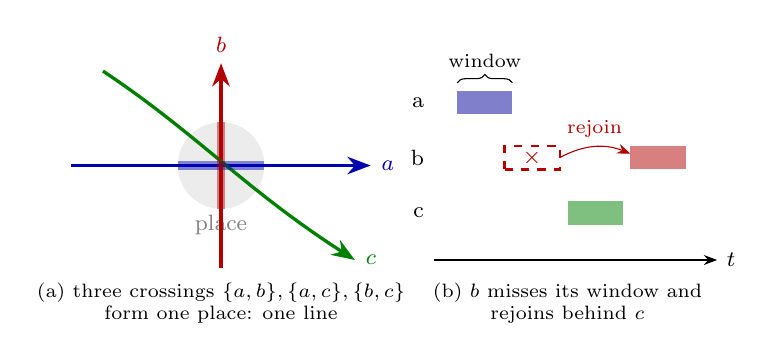
\begin{tikzpicture}[x=1cm,y=1cm,>=Stealth,font=\footnotesize]
  % (a) plan view
  \fill[gray!15] (1.9,1.0) circle (0.55);
  \node[gray] at (1.9,0.25) {place};
  \draw[very thick,->,blue!70!black] (0,1.0) -- (3.8,1.0) node[right] {$a$};
  \draw[very thick,->,red!70!black] (1.9,-0.3) -- (1.9,2.3) node[above] {$b$};
  \draw[very thick,->,green!50!black] (0.4,2.2) .. controls (1.6,1.4) and (2.2,0.7) .. (3.6,-0.2) node[right] {$c$};
  \draw[line width=3pt,blue!70!black,opacity=.45] (1.35,1.0) -- (2.45,1.0);
  \draw[line width=3pt,red!70!black,opacity=.45] (1.9,0.45) -- (1.9,1.55);
  \node[font=\scriptsize,align=center] at (1.9,-0.75) {(a) three crossings $\{a,b\},\{a,c\},\{b,c\}$\\ form one place: one line};
  % (b) time line
  \begin{scope}[xshift=4.6cm]
    \draw[->] (0,-0.2) -- (3.6,-0.2) node[right] {$t$};
    \foreach \y/\n in {1.8/a,1.1/b,0.4/c} \node[left] at (0,\y) {\n};
    % a: token, enters
    \fill[blue!60!black,opacity=.5] (0.3,1.65) rectangle (1.0,1.95);
    % b: window expires
    \draw[red!70!black,dashed,thick] (0.9,0.95) rectangle (1.6,1.25);
    \node[red!70!black] at (1.25,1.1) {$\times$};
    % c: moves ahead
    \fill[green!50!black,opacity=.5] (1.7,0.25) rectangle (2.4,0.55);
    % b rejoins later
    \fill[red!70!black,opacity=.5] (2.5,0.95) rectangle (3.2,1.25);
    \draw[->,red!70!black] (1.6,1.1) to[bend left=25] node[above,font=\scriptsize] {rejoin} (2.5,1.15);
    \draw[decorate,decoration={brace,amplitude=3pt}] (0.3,2.05) -- (1.0,2.05) node[midway,above=2pt,font=\scriptsize] {window};
    \node[font=\scriptsize,align=center] at (1.7,-0.75) {(b) $b$ misses its window and\\ rejoins behind $c$};
  \end{scope}
\end{tikzpicture}
\caption{Crossing queues. (a) Members of the three trucks at one place form
one line. (b) Each member's token opens a window $[t,\;t_{\mathrm{plan}}+
t_{\mathrm{slack}}]$; a member that misses it rejoins at its new free-flow time
if the orders stay lock-free, and the member behind is pulled forward.}
\label{fig:concept}
\end{figure}

\begin{algorithm}[t]
\caption{Traffic manager period (every 1\,s)}
\label{alg:step}
\begin{algorithmic}[1]
\State drop passed crossings; mark entered members
\If{orders locked (abstract execution)} \State heal: move waiting members ahead \EndIf
\For{members past their deadline, not entered}
  \If{held by predecessor} \State renew window
  \Else \State rejoin at new free-flow ticket if lock-free \EndIf
\EndFor
\If{global and $T_{\mathrm{opt}}$ elapsed}
  \State solve (\ref{eq:order})--(\ref{eq:obj}); set open tickets
  \State keep iff lock-free $\wedge$ fixed orders kept $\wedge$ $J$ falls
\EndIf
\State local search: swap tickets of $\le30$ open crossings if $J$ falls
\State issue tokens to members due within $t_{\mathrm{iss}}$
\State per truck: grant end from order conditions and claims; pace (\ref{eq:pace})
\end{algorithmic}
\end{algorithm}

%=============================================================================
\section{Experimental Setup}
\label{sec:setup}
%=============================================================================

\subsection{Floors, disturbances and simulation}
% src: docs/plans/2026-10-09-fleet-random-worlds.md (W0, W3, W4, W5)
A generator turns a seed into one of three floor types: a \emph{rack
warehouse} (hall 70--110$\times$45--70\,m, 2--4 rack blocks, picking aisles
6.8--8.0\,m), a \emph{process shop} (hall 60--100$\times$50--80\,m, column
grid 10--14\,m, machines of 3--9\,m with input and output slots), and a
\emph{multi-hall} plant joining 2--3 such halls through 5--8\,m doors and,
for some seeds, a single-lane connector 4--4.5\,m wide where oncoming trucks
cannot pass. Six conditions are run: C0 (traffic only; 5, 10 or 20 trucks)
and, with 10 trucks, C1 faults (a 30--120\,s stop, a permanent breakdown and
a 1--2\,m spill blocking an aisle), C2 communication (0.5\,s delay, 20\,\%
grant loss), C3 localization (slowly varying bias up to 0.17\,m), C4
pedestrians (10 people at 1.2\,m/s; a truck stops when one is in its
protective field, braking distance $+1$\,m ahead), and C5 (C1--C4 together).
A CPU simulator steps at 0.1\,s for 1{,}800\,s per cell. All policies use the
same vehicle model (Sec.~\ref{sec:milp}, acceleration cap 0.30\,m/s$^2$) and
loads drawn uniformly from 5--13\,kg per job.

\subsection{Policies}
% src: crossing-queues plan (section 4), literature-baselines plan (methods)
Table~\ref{tab:variants} lists the policies. \Qone--\Qthree{} add queues,
pacing and global ordering in turn; B and \Qthreep{} use the physical time
model. The literature methods are mapped onto the same routes and safety
layer, so they decide only order and reservations: L2 (critical sections,
DISTANCE heuristic: the truck closer to the section goes first, revised every
second and changed only where the yielding truck can still stop and the new
orders are acyclic~\cite{pecora2018,mannucci2021}), L3 (ADG: the free-flow
order at route assignment, never changed~\cite{honig2019}), and L4 (prioritized
space--time reservation by job order on fixed routes, 30\,s window re-solved
every 5\,s, executed in crossing order~\cite{li2021rhcr,varambally2022,cap2015}).
Tile reservation~\cite{fransen2022} (L1; 0.25\,m tiles, whole-route
banker's-style check) still had wait cycles over 60\,s in 21 of 40
development cells after three fixes, so it is not compared
here~\todo{add L1 evaluation result if completed}. SADG
re-ordering~\cite{berndt2024} is closest to \Qthree{} and was not
reimplemented.

\begin{table}[t]
\centering
\caption{Policies (all share routes, claims, TA/RA)}
\label{tab:variants}
\footnotesize
\setlength{\tabcolsep}{3pt}
\begin{tabular}{llccl}
\toprule
& Order mechanism & Pace & Re-order & ETA \\
\midrule
A    & time windows, first truck's token & -- & local & simple \\
B    & as A & -- & local & physical \\
\Qone  & crossing queues & -- & local & simple \\
\Qtwo  & crossing queues & yes & local & simple \\
\Qthree  & crossing queues & yes & MILP + local & simple \\
\Qthreep & crossing queues & yes & MILP + local & physical \\
\midrule
L2 & critical sections~\cite{pecora2018,mannucci2021} & -- & heuristic & -- \\
L3 & ADG, fixed order~\cite{honig2019} & -- & none & plan \\
L4 & prioritized reservation~\cite{li2021rhcr,cap2015} & -- & every 5\,s & free + wait \\
\bottomrule
\end{tabular}
\end{table}

\subsection{Protocol and metrics}
% src: crossing-queues plan ("평가 (결과 보기 전 고정)", "평가에서 뺀 칸", "평가 결과")
Parameters ($t_{\mathrm{iss}}=30$\,s, $t_{\mathrm{slack}}=10$\,s,
$\alpha=120$\,s, pace floor 0.1\,m/s, $T_{\mathrm{opt}}=5$\,s, node limit
2{,}000) were left at their initial values on development seeds 100--102. Two
code fixes found there---unmerged members (Sec.~\ref{sec:queues}) and keeping
replanned routes clear of other trucks' claims---were made before the code was
frozen. The evaluation seeds 700--704 give 120 cells (3 floor types
$\times$ 5 seeds $\times$ 8 condition/fleet-size combinations), each run once
per policy. One cell fails floor generation for every policy, and any cell a
policy did not finish within 10\,h of wall time is removed from all policies,
leaving 117 cells. A policy passes if it has zero truck--truck overlaps (ground
truth), no wait cycle longer than 60\,s and no gridlock (no working truck
advancing for 300\,s). We report completed jobs, the number of waits behind
another truck longer than 60 and 300\,s, the longest such wait, the mean share
of truck time spent blocked, stops, and failed RA attempts.

\subsection{Large-scale study}
% src: docs/plans/2026-10-17-fleet-large-random-chained.md
To stress scale, floors are generated with the hall-size ranges $\times1.5$
(area $\times2.25$; e.g.\ rack seed 800: $149.1\times77.2$\,m, 281 slots;
multi-hall seed 800: $257.6\times73.4$\,m, 244 slots) and run with 20 trucks.
Jobs pick a random full slot and drop at a random empty one (60\,\% of slots
initially full), and a truck takes its next job where it dropped the last one
(\emph{chaining}) instead of returning to a holding slot. Seeds 800--805, three
floor types and conditions C0 and C5 give 36 cells per policy, with the
evaluated settings unchanged and a larger planner budget for all policies.
Cells over the 16\,h limit were rerun with a parallel planner that returns the
same plans (identical trajectories on a check cell), so all 36 cells are
compared. Differences in jobs are reported as paired cell bootstrap intervals
(4{,}000 resamples, 95\,\%) of the ratio of job totals.

%=============================================================================
\section{Results}
\label{sec:results}
%=============================================================================

\begin{table}[t]
\centering
\caption{Evaluation, 117 cells (seeds 700--704, sums over cells)}
\label{tab:main}
\footnotesize
\setlength{\tabcolsep}{2.6pt}
% src: crossing-queues plan "평가 결과" table; literature-baselines plan "L2 · L3 · L4 평가 끝" table
\begin{tabular}{lrrrrrrrr}
\toprule
 & Jobs & $>$60\,s & $>$300\,s & Max (s) & Blocked & GL & Stops & RA fail \\
\midrule
A        & 2,982 & 343 & 21 & 540 & 4.9\,\% & 1 & 3,461 & 353 \\
B        & 2,969 & 378 &  4 & 420 & 4.5\,\% & 0 & 3,436 & 285 \\
\Qone    & 2,970 & 394 &  7 & 398 & 5.1\,\% & 0 & 3,732 & 325 \\
\Qtwo    & 2,815 & 385 & 14 & 479 & 3.4\,\% & 0 & 3,730 & 339 \\
\Qthree  & 2,988 &  51 &  0 & 124 & 1.3\,\% & 0 & 3,259 &  24 \\
\Qthreep & 2,971 &  34 &  0 & 120 & 1.3\,\% & 0 & 3,310 &  16 \\
\midrule
L2       & 3,064 & 178 &  0 & 228 & 3.9\,\% & 0 & -- & -- \\
L3       & 2,749 & 794 & 49 & 931 & 8.5\,\% & 2 & -- & -- \\
L4       & 2,896 & 490 & 16 & 630 & 7.8\,\% & 0 & -- & -- \\
\bottomrule
\end{tabular}\\[2pt]
\parbox{\columnwidth}{\scriptsize Waits are behind another truck. GL:
gridlock cells. All policies: zero truck--truck overlaps, no wait cycle
$>$60\,s. --: not tabulated in our records.}
\end{table}

\subsection{117-cell evaluation}
% src: crossing-queues plan "평가 결과"; literature-baselines plan table; derived ratios marked
Table~\ref{tab:main} gives the results. All nine policies kept trucks apart
and none had a wait cycle over 60\,s; A and L3 stopped in gridlock in one and
two cells, L3's being waits on an immobile truck rather than cycles. All five
queue and window variants that are judged (B, \Qone--\Qthreep) passed.

\emph{Ablation.} Queues alone (\Qone) did not help: jobs within 0.4\,\% of A, % derived: 2970/2982
but more long waits and stops. Pacing with local re-ordering (\Qtwo) lowered jobs by
5.2\,\% against \Qone. % derived: 2815/2970
Global re-ordering is what changed the picture: \Qthree{} completed as many jobs
as A (+0.2\,\%) % derived: 2988/2982
while waits over 60\,s fell from 343 to 51 ($-85$\,\%), % derived
waits over 300\,s from 21 to 0, the longest wait from 540\,s to 124\,s, the
blocked share from 4.9\,\% to 1.3\,\%, stops by 5.8\,\% % derived: 3259/3461
and failed RA attempts from 353 to 24. The physical time model did not raise
throughput (B vs.\ A $-0.4$\,\%, \Qthreep{} vs.\ \Qthree{} $-0.6$\,\%), though
\Qthreep{} had fewer long waits (34 vs.\ 51). Throughput differences between
A, B, \Qone, \Qthree{} and \Qthreep{} are within 0.7\,\%, and we did not test
whether they exceed chance. By the prespecified rule (highest throughput among
passing queue variants), \Qthree{} was adopted.

\emph{Literature methods.} The critical-section coordinator L2 completed the
most jobs, 2.5\,\% more than \Qthree, % derived: 3064/2988
but had 3.5 times as many waits over 60\,s and a longest wait of 228\,s.
% derived: 178/51
The fixed order of L3 had the most long waits (794; longest 931\,s), and
priority reservations (L4) made low-priority trucks wait long (490; 630\,s).
The price of \Qthree{} is computation: the MILP took 29{,}931\,s of wall time
over the 117 cells, 256\,s per 1{,}800\,s simulated cell.
% derived: 29931/117

\begin{table}[t]
\centering
\caption{Large-scale study, 36 cells (20 trucks, 1.5$\times$ floors, chaining)}
\label{tab:large}
\footnotesize
\setlength{\tabcolsep}{3pt}
% src: large-random-chained plan "CPU r2 + r2x (216 칸 전부)" table; overlaps from
%      result.json contacts (no "truck" key in any of the 216 runs)
\begin{tabular}{lrrrrrrr}
\toprule
 & Jobs & $>$60\,s & $>$300\,s & Max (s) & Blocked & GL & Cyc$>$60 \\
\midrule
A        & 1,781 & 1,488 & 118 & 1,198 & 21.2\,\% & 0 & 0 \\
\Qone    & 1,658 & 1,450 & 162 & 1,669 & 23.9\,\% & 1 & 2 \\
\Qthree  & 1,929 &   319 &  77 & 1,362 &  9.0\,\% & 1 & 2 \\
\Qthreep & 1,971 &   368 &  63 & 1,509 &  8.4\,\% & 1 & 3 \\
L2       & 1,972 &   690 &  49 & 1,244 & 13.1\,\% & 1 & 2 \\
L4       & 1,791 & 1,075 &  59 & 1,337 & 18.9\,\% & 1 & 1 \\
\bottomrule
\end{tabular}\\[2pt]
\parbox{\columnwidth}{\scriptsize Cyc$>$60: cells with a wait cycle over
60\,s. Zero truck--truck overlaps in all runs. Jobs are counted at chaining
and are not comparable with Table~\ref{tab:main}.}
\end{table}

\begin{table*}[t]
\centering
\caption{Paired differences in completed jobs, large-scale study (\% of the
second policy; cell bootstrap, 4{,}000 resamples, 95\,\% interval)}
\label{tab:boot}
\footnotesize
% src: large-random-chained plan, bootstrap table (36 cells)
\begin{tabular}{lcccc}
\toprule
 & All 36 & Shop 12 & Rack 12 & Multi-hall 12 \\
\midrule
\Qthree{} $-$ A        & $+8.3$ [$1.9$, $15.7$]   & $-2.1$ [$-4.6$, $0.8$] & $+25.6$ [$13.1$, $40.0$] & $+12.9$ [$-7.6$, $31.8$] \\
\Qthree{} $-$ \Qone    & $+16.3$ [$9.4$, $25.5$]  & $+1.3$ [$-2.2$, $5.5$] & $+40.2$ [$25.5$, $59.6$] & $+26.8$ [$10.8$, $46.8$] \\
\Qthree{} $-$ L2       & $-2.2$ [$-8.8$, $3.6$]   & $-2.3$ [$-5.8$, $1.4$] & $+9.9$ [$2.4$, $20.2$]   & $-13.2$ [$-36.0$, $2.4$] \\
\Qthree{} $-$ L4       & $+7.7$ [$2.0$, $12.8$]   & $+4.2$ [$1.1$, $6.9$]  & $+17.8$ [$10.2$, $28.1$] & $+4.0$ [$-16.3$, $19.4$] \\
\Qthreep{} $-$ \Qthree & $+2.2$ [$-4.0$, $11.5$]  & $+0.6$ [$-1.9$, $3.0$] & $-8.1$ [$-13.8$, $-2.6$] & $+17.3$ [$-5.0$, $65.9$] \\
\Qthreep{} $-$ L2      & $-0.1$ [$-3.9$, $4.0$]   & $-1.7$ [$-4.8$, $1.4$] & $+1.0$ [$-4.4$, $9.5$]   & $+1.8$ [$-9.8$, $13.5$] \\
L2 $-$ A               & $+10.7$ [$5.0$, $18.4$]  & $+0.2$ [$-3.7$, $3.7$] & $+14.3$ [$3.9$, $24.2$]  & $+30.1$ [$13.2$, $58.0$] \\
\bottomrule
\end{tabular}
\end{table*}

\subsection{Large-scale study}
% src: large-random-chained plan "CPU r2 + r2x" and "계산 줄이기"
Tables~\ref{tab:large} and~\ref{tab:boot} summarize the 20-truck floors.
\Qthree, \Qthreep{} and L2 completed 8--11\,\% more jobs than A and are
indistinguishable from each other overall (all three pairwise intervals contain
zero). The gains over A come from the rack (\Qthree{} $+25.6$\,\%) and
multi-hall floors; on shop floors \Qthree, \Qthreep, L2 and A are within about 2\,\%.
\Qthree{} beat L2 on rack floors ($+9.9$\,\%) but trailed it on multi-hall
floors ($-13.2$\,\%, interval containing zero). Waits over 60\,s were 0.46 and
0.53 times those of L2 for \Qthree{} and \Qthreep, % derived: 319/690, 368/690
but waits over 300\,s were more frequent (77 and 63 vs.\ 49), mostly on
multi-hall floors (53, 30 and 9).

Unlike the 117-cell evaluation, every policy except A had at least one
gridlock or wait cycle over 60\,s here (Table~\ref{tab:large}). Two \Qthree{}
cells collapsed: multi\_802\_C5\_20 gridlocked at 1{,}443\,s with no job done
(other policies 11--48), and multi\_805\_C5\_20 finished 4 jobs (\Qthreep{} 48,
L2 31). Both started within 1\,s of a spill or fault, when 4--12 trucks
replanned at once and the new routes locked the orders. Healing turns at most
four orders per period and cannot turn crossings already entered; and since a
candidate detour is tested against the whole order set, every detour is
rejected while the orders are locked, which we believe is why RA did not help
(289 and 329 failed RA attempts, against 11 for \Qthreep{} in the same cells).
This diagnosis is from event logs and code; the cells were not rerun. Across all 216 runs, healing succeeded 3 times and failed
11{,}041 times. This mechanism is shared by every policy built on the
crossing orders (A, \Qone, \Qthree, \Qthreep, L2--L4) and also caused the L2
deadlock in rack\_804\_C5\_20. Leaving the two cells out post hoc,
\Qthree{} $-$ L2 becomes $+1.5$\,\% [$-1.9$, $5.3$].

\emph{Computation.} The MILP did not keep up with real time on the larger
floors: per cell (one core of an AMD EPYC 9755 node) it took 439\,s (shop),
10{,}170\,s (rack) and 13{,}792\,s (multi-hall) for 1{,}800\,s simulated, with
a maximum of 50{,}072\,s. On the 21 cells every policy finished within the
first 16\,h, one solve took 1.2, 8.8 and 27.6\,s on average on the three floor
types, against the 5\,s period, and only 34--36\,\% of solves were kept; the
rest raised $J$ or conflicted with fixed orders. In a 600\,s profiling run on
a rack floor, solves had on average 621 binaries and 5{,}136 rows, model
building took about 0.08\,s and the node limit did not bound the solve time.
Restricting the binaries to crossings reached within a horizon of 60 or 120\,s
cut the time 6--20 fold but lost 3.6--7.1\,\% of jobs on those 21 cells, with
intervals below zero, so we did not adopt it.

\begin{figure}[t]
\centering
\fbox{\parbox[c][3.2cm][c]{0.92\columnwidth}{\centering\footnotesize
\todo{Figure: per-cell paired job difference \Qthree{} $-$ A and \Qthree{} $-$
L2 by floor type (36 cells), and wait-length distribution (117 cells).
Data: result.json of eval700 and r2/r2x runs.}}}
\caption{\todo{Per-cell differences and wait distributions.}}
\label{fig:results}
\end{figure}

%=============================================================================
\section{Discussion and Limitations}
%=============================================================================

Most of the benefit of crossing queues comes from the global ordering: queues
and pacing alone did not help, and pacing with only local re-ordering hurt.
The MILP mainly removes long waits rather than adding throughput at the
original scale; at 20 trucks on 2.25 times the area it also adds throughput,
matching a well-tuned critical-section heuristic with fewer waits over 60\,s
but more over 300\,s.

The limitations are substantial. (i) The MILP is not real-time on large
floors with the node-limited solver we used; horizon truncation was too
costly in jobs, and how to bound the solve time without losing its benefit is
open. (ii) Locked orders after simultaneous replanning are not reliably
healed, which collapsed two \Qthree{} cells and affects all crossing-order
policies. (iii) All comparisons are in a CPU simulator with perfect path
tracking; representative runs in NVIDIA Isaac Sim with physical vehicles were
used only for inspection, since single runs differ by chance and pallets
slipped off the forks in transport there (8--14 lowerings without a pallet per
policy on a scaled rack floor), an issue also seen without chaining whose cause
is still open. (iv) Each cell was run once; the 117-cell throughput differences
were not tested for significance. (v) The vehicle parameters beyond the
measured dimensions, load range, pedestrian behaviour and protective field are
estimates or simple models, and truck--pedestrian contacts, recorded but not
judged, occurred under all policies. (vi) Literature methods were adapted to
fixed continuous routes and our safety layer; their published forms assume
grids or roadmaps.

%=============================================================================
\section{Conclusion}
%=============================================================================

Crossing queues give every truck at every place where free-form routes touch
its own ticket, window and token, re-queue late trucks where the order graph
stays acyclic, and re-order all open crossings by a MILP. In 117 generated
cells they kept throughput equal to a time-window baseline while cutting waits
over 60\,s by 85\,\%, without overlaps or deadlocks, and on larger floors with
20 trucks they matched an adapted critical-section coordinator in throughput.
Bounding the solve time and healing locked orders after mass replanning are the
next steps \todo{future work as decided}.

\bibliographystyle{IEEEtran}
\bibliography{refs}

\end{document}
